\documentclass[tikz,border=3pt]{standalone}
\usepackage[utf8]{inputenc}
\usepackage[T1]{fontenc}
\usepackage{lmodern}
\renewcommand{\familydefault}{\sfdefault}
\usepackage{sansmath}\sansmath
\usepackage{chemfig}
\usepackage{pgfplots}\pgfplotsset{compat=1.18,/pgf/number format/use comma,/pgf/number format/1000 sep={.}}
\usetikzlibrary{arrows.meta,calc,positioning,decorations.pathmorphing,patterns}
% paleta del sitio
\definecolor{nar}{HTML}{E8680C}\definecolor{narc}{HTML}{FFB35C}\definecolor{hielo}{HTML}{FFF3E8}
\definecolor{tinta}{HTML}{1D1D1F}\definecolor{gris}{HTML}{6E6E73}\definecolor{lila}{HTML}{7C5CF0}
\definecolor{azul}{HTML}{2F6FD6}\definecolor{menta}{HTML}{17A673}\definecolor{coral}{HTML}{E8342A}
\tikzset{cel/.style={draw=gris,fill=hielo,line width=0.9pt},nuc/.style={draw=gris!70,line width=0.6pt},
fib/.style={gris!55,line width=0.35pt},eti/.style={font=\footnotesize,text=tinta,align=center},
num/.style={circle,draw=nar,fill=white,text=nar,font=\small\bfseries,inner sep=1.2pt,minimum size=13pt},
fl/.style={-{Stealth[length=2.6mm]},gris,line width=0.9pt}}
\begin{document}
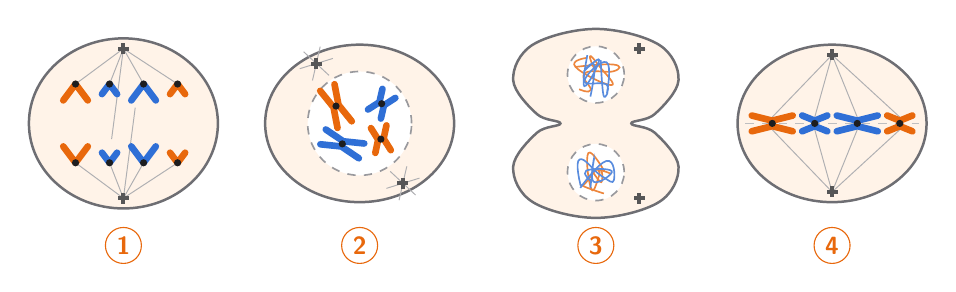
\begin{tikzpicture}[font=\small]
\draw[cel] (0,0) ellipse (1.2 and 1.08);
\draw[fib] (0,0.95)--(-0.608,0.5);
\draw[fib] (0,-0.95)--(-0.608,-0.5);
\draw[fib] (0,0.95)--(-0.176,0.5);
\draw[fib] (0,-0.95)--(-0.176,-0.5);
\draw[fib] (0,0.95)--(0.256,0.5);
\draw[fib] (0,-0.95)--(0.256,-0.5);
\draw[fib] (0,0.95)--(0.688,0.5);
\draw[fib] (0,-0.95)--(0.688,-0.5);
\draw[fib] (0,0.95)--(-0.15,-0.2);
\draw[fib] (0,-0.95)--(0.15,0.2);
\begin{scope}[shift={(-0.608,0.5)},rotate=0]\draw[nar,line width=2.4pt,line cap=round,line join=round] (-0.156,-0.208)--(0,0)--(0.156,-0.208);\end{scope}
\fill[tinta] (-0.608,0.5) circle (1.3pt);
\begin{scope}[shift={(-0.608,-0.5)},rotate=180]\draw[nar,line width=2.4pt,line cap=round,line join=round] (-0.156,-0.208)--(0,0)--(0.156,-0.208);\end{scope}
\fill[tinta] (-0.608,-0.5) circle (1.3pt);
\begin{scope}[shift={(-0.176,0.5)},rotate=0]\draw[azul,line width=2.4pt,line cap=round,line join=round] (-0.096,-0.128)--(0,0)--(0.096,-0.128);\end{scope}
\fill[tinta] (-0.176,0.5) circle (1.3pt);
\begin{scope}[shift={(-0.176,-0.5)},rotate=180]\draw[azul,line width=2.4pt,line cap=round,line join=round] (-0.096,-0.128)--(0,0)--(0.096,-0.128);\end{scope}
\fill[tinta] (-0.176,-0.5) circle (1.3pt);
\begin{scope}[shift={(0.256,0.5)},rotate=0]\draw[azul,line width=2.4pt,line cap=round,line join=round] (-0.156,-0.208)--(0,0)--(0.156,-0.208);\end{scope}
\fill[tinta] (0.256,0.5) circle (1.3pt);
\begin{scope}[shift={(0.256,-0.5)},rotate=180]\draw[azul,line width=2.4pt,line cap=round,line join=round] (-0.156,-0.208)--(0,0)--(0.156,-0.208);\end{scope}
\fill[tinta] (0.256,-0.5) circle (1.3pt);
\begin{scope}[shift={(0.688,0.5)},rotate=0]\draw[nar,line width=2.4pt,line cap=round,line join=round] (-0.096,-0.128)--(0,0)--(0.096,-0.128);\end{scope}
\fill[tinta] (0.688,0.5) circle (1.3pt);
\begin{scope}[shift={(0.688,-0.5)},rotate=180]\draw[nar,line width=2.4pt,line cap=round,line join=round] (-0.096,-0.128)--(0,0)--(0.096,-0.128);\end{scope}
\fill[tinta] (0.688,-0.5) circle (1.3pt);
\fill[tinta!75] (-0.07,0.925) rectangle (0.07,0.975);\fill[tinta!75] (-0.025,0.88) rectangle (0.025,1.02);
\fill[tinta!75] (-0.07,-0.975) rectangle (0.07,-0.925);\fill[tinta!75] (-0.025,-1.02) rectangle (0.025,-0.88);
\draw[cel] (3,0) ellipse (1.2 and 1);
\draw[nuc,fill=white,dashed] (3,0) circle (0.66);
\begin{scope}[shift={(2.7,0.22)},rotate=25]\draw[nar,line width=2.4pt,line cap=round,line join=round] (-0.1,0.26)--(-0.035,0)--(-0.1,-0.26);\end{scope}
\begin{scope}[shift={(2.7,0.22)},rotate=25]\draw[nar,line width=2.4pt,line cap=round,line join=round] (0.1,0.26)--(0.035,0)--(0.1,-0.26);\end{scope}
\fill[tinta] (2.7,0.22) circle (1.3pt);
\begin{scope}[shift={(3.28,0.25)},rotate=-35]\draw[azul,line width=2.4pt,line cap=round,line join=round] (-0.1,0.16)--(-0.035,0)--(-0.1,-0.16);\end{scope}
\begin{scope}[shift={(3.28,0.25)},rotate=-35]\draw[azul,line width=2.4pt,line cap=round,line join=round] (0.1,0.16)--(0.035,0)--(0.1,-0.16);\end{scope}
\fill[tinta] (3.28,0.25) circle (1.3pt);
\begin{scope}[shift={(2.78,-0.26)},rotate=70]\draw[azul,line width=2.4pt,line cap=round,line join=round] (-0.1,0.26)--(-0.035,0)--(-0.1,-0.26);\end{scope}
\begin{scope}[shift={(2.78,-0.26)},rotate=70]\draw[azul,line width=2.4pt,line cap=round,line join=round] (0.1,0.26)--(0.035,0)--(0.1,-0.26);\end{scope}
\fill[tinta] (2.78,-0.26) circle (1.3pt);
\begin{scope}[shift={(3.27,-0.2)},rotate=10]\draw[nar,line width=2.4pt,line cap=round,line join=round] (-0.1,0.16)--(-0.035,0)--(-0.1,-0.16);\end{scope}
\begin{scope}[shift={(3.27,-0.2)},rotate=10]\draw[nar,line width=2.4pt,line cap=round,line join=round] (0.1,0.16)--(0.035,0)--(0.1,-0.16);\end{scope}
\fill[tinta] (3.27,-0.2) circle (1.3pt);
\draw[fib] (2.45,0.76)--(2.66,0.825);
\draw[fib] (2.45,0.76)--(2.499,0.975);
\draw[fib] (2.45,0.76)--(2.289,0.91);
\draw[fib] (2.45,0.76)--(2.24,0.695);
\draw[fib] (2.45,0.76)--(2.401,0.545);
\draw[fib] (2.45,0.76)--(2.611,0.61);
\draw[fib] (3.55,-0.76)--(3.76,-0.695);
\draw[fib] (3.55,-0.76)--(3.599,-0.545);
\draw[fib] (3.55,-0.76)--(3.389,-0.61);
\draw[fib] (3.55,-0.76)--(3.34,-0.825);
\draw[fib] (3.55,-0.76)--(3.501,-0.975);
\draw[fib] (3.55,-0.76)--(3.711,-0.91);
\fill[tinta!75] (2.38,0.735) rectangle (2.52,0.785);\fill[tinta!75] (2.425,0.69) rectangle (2.475,0.83);
\fill[tinta!75] (3.48,-0.785) rectangle (3.62,-0.735);\fill[tinta!75] (3.525,-0.83) rectangle (3.575,-0.69);
\draw[cel] plot[smooth cycle,tension=0.6] coordinates {(6,1.2) (6.8,1) (7.05,0.55) (6.75,0.12) (6.45,0) (6.75,-0.12) (7.05,-0.55) (6.8,-1) (6,-1.2) (5.2,-1) (4.95,-0.55) (5.25,-0.12) (5.55,0) (5.25,0.12) (4.95,0.55) (5.2,1)};
\draw[nuc,fill=white,dashed] (6,0.62) circle (0.36);
\draw[nar!80,line width=0.6pt] plot[smooth,tension=0.9] coordinates {(5.749,0.718) (6.221,0.748) (6.224,0.662) (5.86,0.637) (5.934,0.423) (5.788,0.434)};
\draw[nar!80,line width=0.6pt] plot[smooth,tension=0.9] coordinates {(5.999,0.651) (5.924,0.85) (6.036,0.736) (6.198,0.486) (5.74,0.719) (5.888,0.833)};
\draw[azul!80,line width=0.6pt] plot[smooth,tension=0.9] coordinates {(6.061,0.803) (6.097,0.356) (6.133,0.495) (5.856,0.537) (6.136,0.777) (6.141,0.388)};
\draw[azul!80,line width=0.6pt] plot[smooth,tension=0.9] coordinates {(5.931,0.341) (5.98,0.739) (5.853,0.667) (6.042,0.805) (5.854,0.473) (5.892,0.867)};
\fill[tinta!75] (6.48,0.925) rectangle (6.62,0.975);\fill[tinta!75] (6.525,0.88) rectangle (6.575,1.02);
\draw[nuc,fill=white,dashed] (6,-0.62) circle (0.36);
\draw[nar!80,line width=0.6pt] plot[smooth,tension=0.9] coordinates {(6.197,-0.642) (6.047,-0.596) (6.042,-0.663) (5.943,-0.835) (5.905,-0.376) (6.108,-0.607)};
\draw[nar!80,line width=0.6pt] plot[smooth,tension=0.9] coordinates {(5.956,-0.607) (6.069,-0.746) (6.04,-0.571) (5.865,-0.763) (5.837,-0.794) (6.102,-0.89)};
\draw[azul!80,line width=0.6pt] plot[smooth,tension=0.9] coordinates {(5.947,-0.74) (5.877,-0.601) (6.202,-0.606) (5.972,-0.741) (5.976,-0.449) (5.931,-0.821)};
\draw[azul!80,line width=0.6pt] plot[smooth,tension=0.9] coordinates {(5.807,-0.789) (5.794,-0.457) (6.072,-0.668) (6.228,-0.723) (6.136,-0.476) (5.802,-0.819)};
\fill[tinta!75] (6.48,-0.975) rectangle (6.62,-0.925);\fill[tinta!75] (6.525,-1.02) rectangle (6.575,-0.88);
\draw[cel] (9,0) ellipse (1.2 and 1);
\draw[gris!45,dashed] (7.9,0)--(10.1,0);
\draw[fib] (9,0.87)--(8.24,0.08);
\draw[fib] (9,-0.87)--(8.24,-0.08);
\draw[fib] (9,0.87)--(8.78,0.08);
\draw[fib] (9,-0.87)--(8.78,-0.08);
\draw[fib] (9,0.87)--(9.32,0.08);
\draw[fib] (9,-0.87)--(9.32,-0.08);
\draw[fib] (9,0.87)--(9.86,0.08);
\draw[fib] (9,-0.87)--(9.86,-0.08);
\begin{scope}[shift={(8.24,0)},rotate=90]\draw[nar,line width=2.4pt,line cap=round,line join=round] (-0.1,0.26)--(-0.035,0)--(-0.1,-0.26);\end{scope}
\begin{scope}[shift={(8.24,0)},rotate=90]\draw[nar,line width=2.4pt,line cap=round,line join=round] (0.1,0.26)--(0.035,0)--(0.1,-0.26);\end{scope}
\fill[tinta] (8.24,0) circle (1.3pt);
\begin{scope}[shift={(8.78,0)},rotate=90]\draw[azul,line width=2.4pt,line cap=round,line join=round] (-0.1,0.16)--(-0.035,0)--(-0.1,-0.16);\end{scope}
\begin{scope}[shift={(8.78,0)},rotate=90]\draw[azul,line width=2.4pt,line cap=round,line join=round] (0.1,0.16)--(0.035,0)--(0.1,-0.16);\end{scope}
\fill[tinta] (8.78,0) circle (1.3pt);
\begin{scope}[shift={(9.32,0)},rotate=90]\draw[azul,line width=2.4pt,line cap=round,line join=round] (-0.1,0.26)--(-0.035,0)--(-0.1,-0.26);\end{scope}
\begin{scope}[shift={(9.32,0)},rotate=90]\draw[azul,line width=2.4pt,line cap=round,line join=round] (0.1,0.26)--(0.035,0)--(0.1,-0.26);\end{scope}
\fill[tinta] (9.32,0) circle (1.3pt);
\begin{scope}[shift={(9.86,0)},rotate=90]\draw[nar,line width=2.4pt,line cap=round,line join=round] (-0.1,0.16)--(-0.035,0)--(-0.1,-0.16);\end{scope}
\begin{scope}[shift={(9.86,0)},rotate=90]\draw[nar,line width=2.4pt,line cap=round,line join=round] (0.1,0.16)--(0.035,0)--(0.1,-0.16);\end{scope}
\fill[tinta] (9.86,0) circle (1.3pt);
\fill[tinta!75] (8.93,0.845) rectangle (9.07,0.895);\fill[tinta!75] (8.975,0.8) rectangle (9.025,0.94);
\fill[tinta!75] (8.93,-0.895) rectangle (9.07,-0.845);\fill[tinta!75] (8.975,-0.94) rectangle (9.025,-0.8);
\node[num] at (0,-1.55) {1};
\node[num] at (3,-1.55) {2};
\node[num] at (6,-1.55) {3};
\node[num] at (9,-1.55) {4};
\end{tikzpicture}
\end{document}
